\chapter{Bio-informatica en sequentieanalyse}\label{ch:b3:bioinformatics}

Een bioloog die zojuist een gen van een diepzeeworm heeft gesequenced
plakt zijn \num{300} aminozuren in een webformulier en verneemt drie
seconden later dat het eiwit een verre neef van een menselijk kinase
is, met \qty{31}{\%} identiteit over \num{280} residuen en een kans
$10^{-40}$ dat de gelijkenis toeval is. Achter die drie seconden zitten
een algoritme voor \omterm{thm:b3:bioinformatics:nw}{dynamisch programmeren} uit 1970, een statistische
theorie van toevallige \omterm{def:b3:bioinformatics:alignment}{uitlijningen}, substitutiematrices die uit
duizenden eiwitfamilies zijn gedestilleerd, en een databank van zo'n
honderd miljard residuen. Dit hoofdstuk gaat over de redenering in die
zwarte doos: hoe twee sequenties zo worden uitgelijnd dat de \omterm{def:b3:bioinformatics:alignment}{uitlijning}
aantoonbaar de beste is, hoe de score iets gaat betekenen, hoe een
overeenkomst van een toeval wordt onderscheiden, en hoe patronen worden
gevonden in een genoom waar nog niemand naar heeft gekeken. De wiskunde
is elementair --- een recursie, een logaritme, een poissonverdeling ---
en zij is de moeite waard, omdat elke conclusie uit een
sequentievergelijking erop rust.

\section{Twee sequenties uitlijnen}

\begin{definition}[Uitlijning en score]\label{def:b3:bioinformatics:alignment}
\index{sequentie-uitlijning}\index{hiaatstraf}\index{globale uitlijning}\index{lokale uitlijning}
Een \emph{uitlijning} van twee sequenties schrijft ze boven elkaar, met
\emph{hiaten} (--) ertussen zodat de kolommen een residu met een residu
of een residu met een hiaat paren, en geen enkele kolom twee hiaten
paart. Haar \emph{score} is de som over de kolommen van een
substitutiescore $s(a,b)$ voor elk paar residuen en van een
\emph{hiaatstraf} voor elk hiaat: een lineaire straf $-d$ per
hiaatpositie, of, realistischer, een \emph{affiene} straf
$-d - (k-1)e$ voor een reeks van $k$ hiaten, waarbij de openingskosten
$d$ groter zijn dan de verlengingskosten $e$, omdat één insertie van
verscheidene residuen één enkele evolutionaire gebeurtenis is. Een
\emph{globale} uitlijning beslaat beide sequenties van begin tot eind;
een \emph{lokale} uitlijning zoekt het hoogst scorende paar deelreeksen
en negeert de rest, en dat is wat men wil wanneer een gedeeld domein in
twee verder ongerelateerde eiwitten zit.
\end{definition}

\begin{theorem}[Needleman--Wunsch]\label{thm:b3:bioinformatics:nw}
\index{Needleman--Wunsch}\index{dynamisch programmeren}\index{Smith--Waterman}
Zij $x = x_{1}\dots x_{m}$ en $y = y_{1}\dots y_{n}$, met lineaire
\omterm{def:b3:bioinformatics:alignment}{hiaatstraf} $d$. Definieer $F(i,j)$ als de beste score van een \omterm{def:b3:bioinformatics:alignment}{globale
uitlijning} van de prefixen $x_{1}\dots x_{i}$ en $y_{1}\dots y_{j}$.
Dan geldt $F(i,0) = -id$, $F(0,j) = -jd$, en voor $i,j \ge 1$
\[
F(i,j) = \max\bigl\{\,F(i-1,j-1) + s(x_{i},y_{j}),\;
F(i-1,j) - d,\; F(i,j-1) - d\,\bigr\}.
\]
$F(m,n)$ is de optimale globale score, een optimale \omterm{def:b3:bioinformatics:alignment}{uitlijning} wordt
teruggevonden door vanaf $(m,n)$ de keuzen terug te volgen die elk
maximum opleverden, en de hele berekening kost $mn$ stappen. De
variant van \emph{Smith--Waterman} voor \omterm{def:b3:bioinformatics:alignment}{lokale uitlijning} voegt $0$ als
vierde mogelijkheid aan het maximum toe, zet de randen op $0$ en leest
het antwoord af bij de grootste waarde in de tabel.
\end{theorem}
\begin{proof}
Beschouw de laatste kolom van een willekeurige \omterm{def:b3:bioinformatics:alignment}{uitlijning} van de twee
prefixen. Zij is een van drie dingen: $x_{i}$ boven $y_{j}$, $x_{i}$
boven een hiaat, of een hiaat boven $y_{j}$. Haar weghalen laat een
\omterm{def:b3:bioinformatics:alignment}{uitlijning} over van $(x_{1}\dots x_{i-1},
y_{1}\dots y_{j-1})$, van $(x_{1}\dots x_{i-1}, y_{1}\dots y_{j})$, of van
$(x_{1}\dots x_{i}, y_{1}\dots y_{j-1})$, waarvan de score hoogstens
$F$ van dat paar is; en omgekeerd kan elk van die optimale \omterm{def:b3:bioinformatics:alignment}{uitlijningen}
met de bijbehorende laatste kolom worden verlengd. De beste score die
op elk soort kolom eindigt is dus $F$ van het kortere paar plus de
score van de kolom, en het optimum is de grootste van de drie. De
randen liggen vast (tegenover een leeg prefix zijn alleen hiaten
mogelijk). Inductie naar $i + j$ vult de tabel; het aantal cellen is
$(m+1)(n+1)$. Bij \omterm{def:b3:bioinformatics:alignment}{lokale uitlijning} betekent de extra mogelijkheid $0$
``begin hier een nieuwe \omterm{def:b3:bioinformatics:alignment}{uitlijning}'', wat van $F(i,j)$ de beste score
maakt van een \omterm{def:b3:bioinformatics:alignment}{uitlijning} die \emph{eindigt} op $(i,j)$, en de beste
\omterm{def:b3:bioinformatics:alignment}{lokale uitlijning} eindigt ergens.
\end{proof}

\begin{example}[Een tabel van vier bij drie]\label{ex:b3:bioinformatics:nw-example}
Lijn GAT uit tegen GCAT, met $+1$ voor een overeenkomst, $-1$ voor een
verschil en $d = 1$. De randen zijn $0, -1, -2, -3, -4$ langs de
bovenkant en $0, -1,
-2, -3$ langs de zijkant. Rij voor rij invullen geeft
$F(\text{G},\text{G}) = 1$,
$F(\text{G},\text{C}) = 0$, $F(\text{G},\text{A}) = -1$,
$F(\text{G},\text{T}) = -2$; $F(\text{A},\text{G}) = 0$,
$F(\text{A},\text{C}) = 0$, $F(\text{A},\text{A}) = 1$,
$F(\text{A},\text{T}) = 0$; $F(\text{T},\text{G}) = -1$,
$F(\text{T},\text{C}) = -1$, $F(\text{T},\text{A}) = 0$,
$F(\text{T},\text{T}) = 2$. Het optimum is $2$, en terugvolgen ---
diagonaal vanaf (T,T), diagonaal vanaf (A,A), dan naar links van (G,C)
naar (G,G), dan diagonaal --- geeft
\[
\begin{array}{c}
\texttt{G-AT}\\
\texttt{GCAT}
\end{array}
\]
drie overeenkomsten en één hiaat: $3 - 1 = 2$.
\end{example}

\begin{omfigure}
\begin{tikzpicture}[every node/.style={font=\small}, >=stealth]
  \def\dx{1.0}\def\dy{0.8}
  % headers
  \foreach \j/\c in {1/G,2/C,3/A,4/T} \node[omDef, font=\small\bfseries] at (\j*\dx+0.5,0.4) {\c};
  \foreach \i/\c in {1/G,2/A,3/T} \node[omDef, font=\small\bfseries] at (-0.5,-\i*\dy-0.4) {\c};
  % grid
  \draw[gray!60] (0,0) grid[xstep=\dx, ystep=\dy] (5*\dx,-4*\dy);
  % values
  \foreach \i/\j/\v in {0/0/0,0/1/-1,0/2/-2,0/3/-3,0/4/-4,1/0/-1,2/0/-2,3/0/-3, 1/1/1,1/2/0,1/3/-1,1/4/-2, 2/1/0,2/2/0,2/3/1,2/4/0, 3/1/-1,3/2/-1,3/3/0,3/4/2}
    \node at (\j*\dx+0.5,-\i*\dy-0.4) {$\v$};
  % traceback path highlighted
  \foreach \i/\j in {0/0,1/1,1/2,2/3,3/4} \draw[omThm, very thick] (\j*\dx+0.05,-\i*\dy-0.05) rectangle (\j*\dx+\dx-0.05,-\i*\dy-\dy+0.05);
  \draw[->, omThm, very thick, shorten >=8pt, shorten <=8pt] (4.5,-2.8) -- (3.5,-2.0);
  \draw[->, omThm, very thick, shorten >=8pt, shorten <=8pt] (3.5,-2.0) -- (2.5,-1.2);
  \draw[->, omThm, very thick, shorten >=8pt, shorten <=8pt] (2.5,-1.2) -- (1.5,-1.2);
  \draw[->, omThm, very thick, shorten >=8pt, shorten <=8pt] (1.5,-1.2) -- (0.5,-0.4);
  \node[right, align=left] at (5.6,-1.6) {terugpad vanaf $F(3,4) = 2$:\\diagonaal, diagonaal,\\links (hiaat in GAT), diagonaal\\[3pt] \texttt{G-AT}\\\texttt{GCAT}};
\end{tikzpicture}

{\small De tabel van Needleman--Wunsch voor GAT tegen GCAT
(overeenkomst $+1$, verschil $-1$, hiaat $-1$). Elke cel is de beste
score voor de twee prefixen die daar eindigen; het rode pad dat vanuit
de hoek is teruggevolgd is de optimale \omterm{def:b3:bioinformatics:alignment}{uitlijning}.}
\end{omfigure}

\begin{method}[Twee sequenties uitlijnen]\label{met:b3:bioinformatics:align}
\index{terugpad}
(1) Kies de scoring: een \omterm{def:b3:bioinformatics:matrices}{substitutiematrix} die past bij de verwachte
divergentie (BLOSUM62 voor eiwitten op onbekende afstand,
overeenkomst/verschil voor DNA) en affiene hiaatstraffen (met BLOSUM62
meestal openen $-11$, verlengen $-1$). (2) Beslis globaal of lokaal:
globaal voor twee sequenties die over hun hele lengte homoloog worden
geacht, lokaal in de overige gevallen. (3) Vul de tabel met de
recursie, en bewaar bij elke cel een verwijzing naar de keuze die haar
maximum gaf. (4) Volg terug vanaf $(m,n)$ (globaal) of vanaf de
maximale cel tot een nul (lokaal), en schrijf de \omterm{def:b3:bioinformatics:alignment}{uitlijning} van rechts
naar links. (5) Beoordeel het resultaat niet naar zijn ruwe score maar
naar zijn statistische significantie (hieronder), en kijk ernaar: lange
hiaten, reeksen met weinig complexiteit en \omterm{def:b3:bioinformatics:alignment}{uitlijningen} die tot een
herhaling beperkt blijven zijn waarschuwingen.
\end{method}

\section{Scoren: wat een overeenkomst waard is}

\begin{definition}[Substitutiematrices]\label{def:b3:bioinformatics:matrices}
\index{substitutiematrix}\index{BLOSUM}\index{PAM}\index{log-oddsscore}
Een \emph{substitutiematrix} geeft $s(a,b)$ voor elk paar aminozuren als
een \emph{log-oddsscore}:
\[
s(a,b) = \frac{1}{\lambda}\,\log\frac{q_{ab}}{p_{a}\,p_{b}},
\]
waarin $q_{ab}$ de frequentie is waarmee $a$ en $b$ uitgelijnd worden
aangetroffen in betrouwbare \omterm{def:b3:bioinformatics:alignment}{uitlijningen} van verwante eiwitten,
$p_{a} p_{b}$ de frequentie waarmee zij door toeval zouden worden
gepaard, en $\lambda$ een schaal die zo is gekozen dat de waarden
handige gehele getallen worden. Een positieve score betekent dat het
paar vaker in homologen voorkomt dan door toeval; de identiteitsscores
zijn het grootst voor zeldzame aminozuren (tryptofaan $+11$, cysteïne
$+9$ in BLOSUM62) en het kleinst voor veelvoorkomende (leucine $+4$,
alanine $+4$), en behoudende substituties (isoleucine--valine $+3$)
scoren positief terwijl ingrijpende (tryptofaan--glycine $-2$) negatief
scoren. De \emph{PAM}-matrices (Dayhoff, 1978) werden afgeleid uit nauw
verwante eiwitten en door matrixvermenigvuldiging naar grotere
afstanden geëxtrapoleerd; de \emph{BLOSUM}-matrices (Henikoff en
Henikoff, 1992) werden rechtstreeks geteld in blokken uitgelijnde
sequenties die op een gegeven identiteit waren geclusterd --- BLOSUM62
uit blokken bij \qty{62}{\%} --- en zij zijn de standaard omdat zij
gemeten zijn en niet geëxtrapoleerd, op de afstand waar zij worden
gebruikt.
\end{definition}

\begin{proposition}[Waarom log-odds]\label{prop:b3:bioinformatics:logodds}
\index{verwachte score}
Wil een scoringsschema bij \omterm{def:b3:bioinformatics:alignment}{lokale uitlijning} bruikbaar zijn, dan moet de
\omterm{prop:b3:bioinformatics:logodds}{verwachte score} van een willekeurig gepaarde kolom,
$\sum_{a,b} p_{a} p_{b}\, s(a,b)$, negatief zijn en moeten sommige
scores positief zijn; anders zouden toevallige \omterm{def:b3:bioinformatics:alignment}{uitlijningen}
onbegrensd groeien en zou het hoogst scorende segment de hele sequentie
zijn. Onder die voorwaarde is elk zulk schema gelijkwaardig aan een
log-oddsschema voor \emph{zekere} doelfrequenties $q_{ab}$ --- de
\omterm{def:b3:bioinformatics:alignment}{uitlijningen} die het als optimaal zal vinden zijn die waarvan de
residuparen als $q_{ab}$ zijn verdeeld. De matrix kiezen is dus de
divergentie kiezen die men verwacht op te sporen: een matrix voor nauwe
verwanten (BLOSUM80, PAM30) heeft scherpere positieve en hardere
negatieve waarden, een matrix voor verre verwanten (BLOSUM45, PAM250)
is vlakker.
\end{proposition}
\admitted

\begin{example}[Identiteit, gelijkenis en de schemerzone]\label{ex:b3:bioinformatics:twilight}
Twee willekeurige eiwitsequenties die optimaal met hiaten worden
uitgelijnd halen door toeval ongeveer \qtyrange{15}{20}{\%}
identiteit. Boven \qty{35}{\%} identiteit over honderd residuen zijn
twee eiwitten vrijwel zeker homoloog; tussen \qty{20}{\%} en
\qty{35}{\%} ligt de \emph{schemerzone}, waar identiteit alleen niets
kan beslissen en de statistiek hieronder dat moet doen. Homologen
kunnen ver onder de zone vallen: de subeenheden van hemoglobine en
myoglobine delen \qty{25}{\%} identiteit, lysozym en
$\alpha$-lactalbumine \qty{40}{\%}, en veel paren eiwitten met dezelfde
vouwing delen minder dan \qty{15}{\%}, alleen op te sporen door
\omterm{def:b3:bioinformatics:msa}{profielen} of structuren te vergelijken.
\end{example}

\section{Een databank doorzoeken}

\begin{definition}[BLAST]\label{def:b3:bioinformatics:blast}
\index{BLAST}\index{seed}\index{hoogscorend segmentpaar}
Een zoekvraag van \num{300} residuen tegen een databank van $10^{11}$
uitlijnen met volledig \omterm{thm:b3:bioinformatics:nw}{dynamisch programmeren} zou $3\times 10^{13}$
celbewerkingen per zoekactie kosten. \emph{BLAST} (Altschul en
collega's, 1990) ruilt een beetje gevoeligheid in voor duizendvoudige
snelheid met drie stappen: (1) maak een lijst van de \emph{woorden} van
de zoekvraag (drie residuen voor eiwitten, elf basen voor DNA) en van
hun hoogscorende buren; (2) doorzoek de databank op exacte
woordtreffers --- de \emph{seeds}; (3) verleng elke seed in beide
richtingen zonder hiaten tot de score een vastgestelde hoeveelheid
onder haar beste waarde zakt, en houd de \emph{hoogscorende
segmentparen} (HSP's) over, en verbind daarna nabije HSP's met gehiaat
\omterm{thm:b3:bioinformatics:nw}{dynamisch programmeren} in een smalle band. Een echte homoloog bevat
vrijwel altijd minstens één exact woord van drie residuen; een
toevallige gelijkenis zelden, en die wordt nooit verlengd.
\end{definition}

\begin{omfigure}
\begin{tikzpicture}[every node/.style={font=\scriptsize}, >=stealth]
  % query and database sequences as bars
  \draw[very thick, omDef] (0,2.0) -- (5,2.0); \node[left] at (-0.1,2.0) {zoekvraag};
  \draw[very thick, gray] (0,0.6) -- (11,0.6); \node[left] at (-0.1,0.6) {databank};
  % seeds
  \foreach \q/\d in {1.2/3.6, 2.8/5.2, 4.1/9.3} {
    \fill[omThm] (\q-0.15,1.9) rectangle (\q+0.15,2.1);
    \fill[omThm] (\d-0.15,0.5) rectangle (\d+0.15,0.7);
    \draw[omThm, thick] (\q,1.85) -- (\d,0.75);
  }
  \node[above] at (1.2,2.15) {woord}; \node[above] at (2.8,2.15) {woord}; \node[above] at (4.1,2.15) {woord};
  % extension of the first two (same diagonal) -> HSP
  \draw[<->, very thick, omMeth!70!black] (2.6,0.3) -- (6.2,0.3); \node[below] at (4.4,0.25) {verleng zonder hiaten: een HSP};
  % third seed: extension fails
  \draw[omProp, thick, dashed] (8.8,0.3) -- (9.8,0.3); \node[below, omProp] at (9.3,0.25) {score zakt: verworpen};
  \node[right, align=left] at (5.5,2.0) {1. woorden van de zoekvraag\\2. exacte treffers in de databank (seeds)\\3. verlengen, hoogscorende paren houden};
\end{tikzpicture}

{\small De heuristiek van \omterm{def:b3:bioinformatics:blast}{BLAST}. Korte exacte woorden die de zoekvraag
en een databankvermelding delen (rood) zijn \omterm{def:b3:bioinformatics:blast}{seeds}; elk wordt langs zijn
diagonaal verlengd zolang de score blijft stijgen, en alleen
verlengingen die hoog blijven worden hoogscorende segmentparen.}
\end{omfigure}

\begin{theorem}[De statistiek van een toevallige treffer]\label{thm:b3:bioinformatics:evalue}
\index{E-waarde}\index{bitscore}\index{Karlin--Altschul}
Voor een zoekvraag van lengte $m$ die wordt doorzocht tegen een
databank van totale lengte $n$, met een scoringsschema waarvan de
\omterm{prop:b3:bioinformatics:logodds}{verwachte score} negatief is, is het aantal ongehiaatte \omterm{def:b3:bioinformatics:alignment}{lokale
uitlijningen} met een score van minstens $S$ dat door toeval ontstaat
poissonverdeeld met gemiddelde
\[
E = K\,m\,n\,e^{-\lambda S},
\]
waarin $\lambda$ en $K$ alleen van het scoringsschema en de
residufrequenties afhangen ($\lambda$ is de schaal van de
log-oddsmatrix). $E$ is de \emph{verwachtingswaarde} van de score $S$.
Schrijft men de score in \emph{bits}, $S' = (\lambda S - \ln K)/\ln 2$,
dan wordt de formule $E = m n\, 2^{-S'}$, en de kans dat minstens één
toevallige \omterm{def:b3:bioinformatics:alignment}{uitlijning} $S$ haalt is $P = 1 - e^{-E}$, wat gelijk is aan
$E$ wanneer $E$ klein is.
\end{theorem}
\begin{proof}[Gedeeltelijk bewijs]
De exponentiële staart is de stelling van Karlin--Altschul en wordt
aangenomen: de maximale segmentscore van een toevalswandeling met
negatieve drift heeft een verdeling waarvan de staart als
$e^{-\lambda S}$ afneemt, met $\lambda$ de positieve wortel van
$\sum_{a,b} p_{a} p_{b} e^{\lambda s(a,b)} = 1$ --- en dat is precies
de vergelijking die de log-oddsmatrix consistent maakt. Gegeven die
staart is de rest tellen. Hoogscorende segmenten kunnen bij elk van de
$mn$ paren posities beginnen, zij zijn zeldzaam en zij zijn vrijwel
onafhankelijk; het aantal dat $S$ overtreft is dus poissonverdeeld met
een gemiddelde dat evenredig is met $mn$ en met de staartkans,
$E = Kmn\,e^{-\lambda S}$. De kans op geen enkele is $e^{-E}$. De
vervanging door de \omterm{thm:b3:bioinformatics:evalue}{bitscore} is algebra: $e^{-\lambda S} K = 2^{-(\lambda S -
\ln K)/\ln 2}$. Voor gehiaatte \omterm{def:b3:bioinformatics:alignment}{uitlijningen} geldt dezelfde vorm met
$\lambda$ en $K$ uit simulatie geschat.
\end{proof}

\begin{example}[Een E-waarde lezen]\label{ex:b3:bioinformatics:evalue}
Een zoekvraag van \num{250} residuen tegen een databank van
$5\times 10^{10}$ residuen heeft $mn = 1.25\times 10^{13} \approx 2^{43.5}$.
Een treffer met een \omterm{thm:b3:bioinformatics:evalue}{bitscore} van $60$ heeft
$E = 2^{43.5 - 60} = 2^{-16.5} \approx 10^{-5}$: vrijwel zeker een
homoloog. Een treffer met $S' = 40$ heeft $E = 2^{3.5}
\approx 11$: elf zulke scores zijn door toeval te verwachten, en de
treffer betekent niets. \emph{Dezelfde} \omterm{def:b3:bioinformatics:alignment}{uitlijning}, met dezelfde
\omterm{thm:b3:bioinformatics:evalue}{bitscore}, tegen een tien keer grotere databank doorzocht, heeft een
tien keer grotere $E$ --- significantie is een eigenschap van de
zoekactie, niet van het paar. De gangbare drempel is $E < 10^{-3}$ voor
een betrouwbare homoloog; $E \approx 0.01$--$1$ verdient een tweede
blik met een profielmethode.
\end{example}

\begin{omfigure}
\begin{tikzpicture}
\begin{axis}[
  width=0.7\linewidth, height=5.6cm,
  axis x line=bottom, axis y line=left,
  xmin=25, xmax=70, ymin=0.000000001, ymax=100000000, ymode=log,
  xlabel={bitscore $S'$}, ylabel={$E$},
  xlabel style={font=\small, at={(axis description cs:0.5,-0.12)}, anchor=north},
  ylabel style={font=\small},
  tick label style={font=\small}, xtick={30,40,50,60,70},
  clip=false,
]
\addplot[very thick, omDef, domain=25:70, samples=2] {2^(43.5-x)};
\addplot[very thick, omThm, domain=25:70, samples=2] {2^(46.8-x)};
\addplot[dashed, gray, domain=25:70, samples=2] {0.001};
\node[font=\scriptsize, gray, anchor=south west] at (axis cs:25.5,0.0012) {$E = 10^{-3}$};
\node[font=\scriptsize, omDef, anchor=north west] at (axis cs:26,0.00002) {$mn = 1.25\times 10^{13}$};
\node[font=\scriptsize, omThm, anchor=south west] at (axis cs:45,30) {$mn$ tien keer groter};
\end{axis}
\end{tikzpicture}

{\small $E = mn\,2^{-S'}$: elke extra bit halveert het verwachte aantal
toevallige treffers, en een tien keer grotere databank kost $3.3$ bits
significantie voor dezelfde \omterm{def:b3:bioinformatics:alignment}{uitlijning}.}
\end{omfigure}

\section{Profielen, verborgen toestanden en motieven}

\begin{definition}[Meervoudige uitlijning en profielen]\label{def:b3:bioinformatics:msa}
\index{meervoudige sequentie-uitlijning}\index{profiel}\index{profiel-HMM}
Een \emph{meervoudige \omterm{def:b3:bioinformatics:alignment}{sequentie-uitlijning}} zet een familie van
sequenties in kolommen van homologe residuen. Exact \omterm{thm:b3:bioinformatics:nw}{dynamisch
programmeren} over $k$ sequenties kost $n^{k}$ en is voorbij drie
onmogelijk; praktische programma's lijnen \emph{stapsgewijs} uit,
eerst het naaste paar volgens een gidsboom, daarna sequenties en
groepen bij de groeiende \omterm{def:b3:bioinformatics:alignment}{uitlijning}, met ronden van verfijning. Een
voltooide \omterm{def:b3:bioinformatics:alignment}{uitlijning} wordt samengevat als een \emph{profiel}: per
kolom de frequentie van elk residu en van hiaten. Een
\emph{profiel-HMM}, een verborgen markovmodel, formaliseert dit als een
keten van overeenkomsttoestanden, één per geconserveerde kolom, die elk
residuen met hun eigen kansen uitzenden, met invoeg- en
verwijdertoestanden die op elke positie extra of ontbrekende residuen
toelaten; het model van een familie (een Pfam-vermelding) scoort een
nieuwe sequentie met de kans van het beste pad door de toestanden, en
vindt homologen ver onder de schemerzone van de paarsgewijze
vergelijking, omdat een kolom die alleen hydrofobe residuen duldt dat
ook zegt, terwijl één enkele sequentie dat niet kan.
\end{definition}

\begin{omfigure}
\begin{tikzpicture}[every node/.style={font=\scriptsize}, >=stealth]
  % match states
  \foreach \i in {1,2,3,4} { \draw[thick, fill=omDef!25] (2.2*\i-0.5,0) rectangle (2.2*\i+0.5,0.7); \node at (2.2*\i,0.35) {M$_{\i}$}; }
  % insert states (diamonds) above
  \foreach \i in {1,2,3} { \draw[thick, fill=omProp!30] (2.2*\i+1.1,1.6) -- (2.2*\i+1.55,2.05) -- (2.2*\i+1.1,2.5) -- (2.2*\i+0.65,2.05) -- cycle; \node at (2.2*\i+1.1,2.05) {I$_{\i}$}; }
  % delete states (circles) below
  \foreach \i in {2,3} { \draw[thick, fill=gray!20] (2.2*\i,-1.3) circle (0.4); \node at (2.2*\i,-1.3) {D$_{\i}$}; }
  % transitions match->match
  \foreach \i in {1,2,3} \draw[->, thick] (2.2*\i+0.5,0.35) -- (2.2*\i+1.7,0.35);
  % match->insert->match
  \foreach \i in {1,2,3} { \draw[->, thick, omProp] (2.2*\i+0.3,0.7) -- (2.2*\i+0.9,1.65); \draw[->, thick, omProp] (2.2*\i+1.3,1.65) -- (2.2*\i+1.9,0.7); \draw[->, thick, omProp] (2.2*\i+1.1,2.5) arc[start angle=200, end angle=-20, radius=0.3]; }
  % match->delete->match
  \draw[->, thick, gray] (2.2+0.3,0) -- (4.4-0.3,-1.0); \draw[->, thick, gray] (4.4+0.3,-1.0) -- (6.6-0.3,0); \draw[->, thick, gray] (4.4+0.4,-1.3) -- (6.6-0.4,-1.3); \draw[->, thick, gray] (6.6+0.3,-1.0) -- (8.8-0.3,0);
  \node[below, align=center] at (2.2,-1.2) {emissies: één residuverdeling\\per overeenkomsttoestand};
  \node[right, align=left] at (9.6,1.2) {een sequentie scoort met\\haar beste pad: overeenkomsten,\\invoegingen (oranje) en\\verwijderingen (grijs)};
\end{tikzpicture}

{\small Een \omterm{def:b3:bioinformatics:msa}{profiel-HMM} van een familie met vier kolommen. Elke
overeenkomsttoestand M zendt een residu uit met de eigen frequenties
van de kolom; invoegtoestanden I (met zelflussen) laten extra residuen
toe, verwijdertoestanden D slaan een kolom over. Een sequentie scoren
is haar meest waarschijnlijke pad zoeken.}
\end{omfigure}

\begin{definition}[Motieven en informatie-inhoud]\label{def:b3:bioinformatics:motif}
\index{motief}\index{positiegewichtsmatrix}\index{informatie-inhoud}\index{sequentielogo}
Een \emph{motief} is een kort patroon --- een bindingsplaats voor een
transcriptiefactor, een splitssignaal, een fosforyleringsplaats ---
weergegeven door een \emph{positiegewichtsmatrix} van de frequentie
$f_{i}(b)$ van elke base of elk residu $b$ op elke positie $i$. De
\emph{informatie-inhoud} van positie $i$ is $R_{i} = 2 - H_{i}$ bits
voor DNA, waarbij $H_{i} =
-\sum_{b} f_{i}(b)\log_{2} f_{i}(b)$ haar entropie is: $2$ bits voor
een onveranderlijke base, $0$ voor een positie waar alle vier even
waarschijnlijk zijn. Het totaal $R = \sum_{i} R_{i}$ wordt getekend als
een \emph{sequentielogo}, waarbij elke positie een stapel letters is
waarvan de totale hoogte $R_{i}$ is en waarvan de letters op frequentie
zijn geschaald.
\end{definition}

\begin{proposition}[Hoeveel informatie een plaats nodig heeft]\label{prop:b3:bioinformatics:bits}
\index{informatie-inhoud!en genoomgrootte}
Een plaats die $\gamma$ keer in een genoom van $G$ posities moet worden
gevonden, en nergens anders, heeft ongeveer
$R_{\text{nodig}} = \log_{2}(G/\gamma)$ bits \omterm{def:b3:bioinformatics:motif}{informatie-inhoud} nodig:
het \omterm{def:b3:bioinformatics:motif}{motief} moet de $G$ kandidaatposities tot de $\gamma$ echte
terugbrengen, en elke bit halveert het aantal kandidaten. De waargenomen
motieven van goed onderzochte bacteriële regulatoren voldoen aan die
voorspelling --- plaatsen in \emph{E.~coli} voor een repressor die
enkele tientallen plekken in een genoom van \qty{4.6}{Mb} bindt dragen
\numrange{16}{18} bits; motieven van eukaryote transcriptiefactoren,
met \numrange{8}{12} bits in een genoom van $3\times 10^{9}$, kunnen
hun doelwitten niet alleen aanwijzen, en daarom werken zij in
combinaties en in het open \omterm{def:b3:chromatin-epigenetics:nucleosome}{chromatine} van
\cref{ch:b3:chromatin-epigenetics}.
\end{proposition}
\begin{proof}
Een willekeurige positie past op een \omterm{def:b3:bioinformatics:motif}{motief} met \omterm{def:b3:bioinformatics:motif}{informatie-inhoud} $R$
met kans ongeveer $2^{-R}$ (elke bit specificiteit halveert de kans),
dus is het verwachte aantal toevallige treffers in $G$ posities
$G\,2^{-R}$. Willen de echte plaatsen eruit springen, dan moet dit van
de orde $\gamma$ of kleiner zijn: $G\,2^{-R} \le \gamma$, dat wil
zeggen $R \ge \log_{2}(G/\gamma)$.
\end{proof}

\begin{example}[Verwachte toevallige treffers]\label{ex:b3:bioinformatics:motif-numbers}
Een restrictieplaats van zes vaste basen heeft $R = 12$ bits en past op
een willekeurige positie met kans $4^{-6} = 2^{-12}$: ongeveer
\num{1100} keer in een genoom van \emph{E.~coli} van \qty{4.6}{Mb} op
beide strengen gelezen (de plaats is palindroom, dus één keer per
positie), en $7\times 10^{5}$ keer in het menselijk genoom. Een
eukaryote factor waarvan het \omterm{def:b3:bioinformatics:motif}{motief} $10$ bits draagt past op
$3\times 10^{9}\times 2^{-10} \approx 3$ miljoen posities in het
menselijk genoom, enkele duizenden keren meer dan de genen die zij
reguleert. Een \omterm{def:b3:bioinformatics:motif}{motief} alleen is een zwakke voorspeller in een groot
genoom; de toestand van het \omterm{def:b3:chromatin-epigenetics:nucleosome}{chromatine}, de naburige motieven en de
conservering van de plaats tussen soorten maken pas een voorspelling.
\end{example}

\begin{omfigure}
\begin{tikzpicture}[every node/.style={font=\scriptsize}]
  % sequence logo: TATA box-like 8 positions, stack heights = information content (1 bit = 1 cm)
  \draw[->] (0,0) -- (0,2.2); \node[left] at (-0.05,2.0) {2}; \node[left] at (-0.05,1.0) {1}; \node[left] at (-0.05,0) {0}; \node[rotate=90, above] at (-0.55,1.1) {bits};
  \draw (0,0) -- (8.6,0);
  \node[anchor=south, inner sep=0] at (0.5,0) {\resizebox{0.6cm}{1.9cm}{\textcolor{omThm}{\bfseries T}}};
  \node[anchor=south, inner sep=0] at (1.5,0) {\resizebox{0.6cm}{1.9cm}{\textcolor{omMeth!70!black}{\bfseries A}}};
  \node[anchor=south, inner sep=0] at (2.5,0) {\resizebox{0.6cm}{1.7cm}{\textcolor{omThm}{\bfseries T}}};
  \node[anchor=south, inner sep=0] at (3.5,0) {\resizebox{0.6cm}{1.9cm}{\textcolor{omMeth!70!black}{\bfseries A}}};
  \node[anchor=south, inner sep=0] at (4.5,0) {\resizebox{0.6cm}{1.0cm}{\textcolor{omMeth!70!black}{\bfseries A}}};
  \node[anchor=south, inner sep=0] at (4.5,1.0) {\resizebox{0.6cm}{0.4cm}{\textcolor{omThm}{\bfseries T}}};
  \node[anchor=south, inner sep=0] at (5.5,0) {\resizebox{0.6cm}{1.3cm}{\textcolor{omMeth!70!black}{\bfseries A}}};
  \node[anchor=south, inner sep=0] at (5.5,1.3) {\resizebox{0.6cm}{0.3cm}{\textcolor{omThm}{\bfseries T}}};
  \node[anchor=south, inner sep=0] at (6.5,0) {\resizebox{0.6cm}{0.5cm}{\textcolor{omProp}{\bfseries G}}};
  \node[anchor=south, inner sep=0] at (6.5,0.5) {\resizebox{0.6cm}{0.3cm}{\textcolor{omMeth!70!black}{\bfseries A}}};
  \node[anchor=south, inner sep=0] at (7.5,0) {\resizebox{0.6cm}{0.3cm}{\textcolor{omProp}{\bfseries G}}};
  \foreach \i in {1,...,8} \node[below] at (\i-0.5,-0.05) {\i};
  \node[below] at (4.3,-0.5) {positie in de plaats};
\end{tikzpicture}

{\small Een \omterm{def:b3:bioinformatics:motif}{sequentielogo} van een promotormotief van het TATA-boxtype.
De hoogte van elke stapel is de \omterm{def:b3:bioinformatics:motif}{informatie-inhoud} van die positie,
$2 - H_{i}$ bits; de eerste vier posities zijn vrijwel onveranderlijk
en dragen het grootste deel van de ongeveer $12$ bits van het \omterm{def:b3:bioinformatics:motif}{motief}.}
\end{omfigure}

\section{Van sequentie naar functie}

\begin{method}[Een onbekend eiwit annoteren]\label{met:b3:bioinformatics:annotate}
\index{domein}\index{orthologiebepaling}
Gegeven een nieuwe coderende sequentie: (1) vertaal haar in het juiste
leesraam en kijk of er een signaalpeptide, transmembraansegmenten en
gebieden met weinig complexiteit zijn; (2) doorzoek de
eiwitdatabanken met \omterm{def:b3:bioinformatics:blast}{BLAST} en lees de treffers met $E < 10^{-3}$, en let
erop of de \omterm{def:b3:bioinformatics:alignment}{uitlijning} het hele eiwit beslaat (een echte \omterm{def:b3:genomics:comparative}{ortholoog}) of
een segment (een gedeeld domein); (3) doorzoek de domeindatabanken met
\omterm{def:b3:bioinformatics:msa}{profiel-HMM}'s, die families vinden die \omterm{def:b3:bioinformatics:blast}{BLAST} mist en die het eiwit in
domeinen verdelen; (4) leid orthologie af, niet enkel gelijkenis, door
na te gaan of de beste treffer in het andere genoom de zoekvraag als
\emph{zijn} beste treffer heeft (wederzijds beste treffers) of door het
eiwit in een genboom te plaatsen (\cref{ch:b3:molecular-evolution});
(5) draag de functie van \omterm{def:b3:genomics:comparative}{orthologen} behoedzaam over --- een
geconserveerd katalytisch residu pleit voor dezelfde chemie, een
ontbrekend ertegen --- en voorspel de structuur; (6) behandel elke
voorspelling als een hypothese voor de werkbank.
\end{method}

\begin{proposition}[Structuur uit sequentie]\label{prop:b3:bioinformatics:structure}
\index{structuurvoorspelling}\index{homologiemodellering}\index{co-evolutie}
De vouwing van een eiwit wordt bepaald door zijn sequentie
(\cref{ch:b3:structural-biology}), en haar uit de sequentie berekenen
was vijftig jaar lang het centrale onopgeloste probleem van het vak.
Drie benaderingen slaagden na elkaar. \emph{\omterm{prop:b3:bioinformatics:structure}{Homologiemodellering}} bouwt
de structuur van een eiwit op die van een opgeloste homoloog, en dat
gaat betrouwbaar boven \qty{30}{\%} identiteit. \emph{Co-evolutieanalyse}
maakt gebruik van het feit dat twee residuen die in de vouwing contact
maken over een diepe meervoudige \omterm{def:b3:bioinformatics:alignment}{uitlijning} geneigd zijn samen te
muteren, zodat statistisch gekoppelde paren kolommen voorspelde
contacten zijn, en genoeg contacten leggen een vouwing vast. Methoden
uit het diepe leren, getraind op de honderdduizend opgeloste structuren
en op zulke \omterm{def:b3:bioinformatics:alignment}{uitlijningen}, voorspellen de meeste bolvormige
eiwitstructuren nu met bijna experimentele nauwkeurigheid (de
CASP-beoordelingen van 2020), en databanken bevatten een voorspelde
structuur voor vrijwel elke bekende eiwitsequentie. Wat zij minder goed
voorspellen is wat één enkele structuur niet vat: wanordelijke
gebieden, andere conformaties, het effect van een puntmutatie en
complexen.
\end{proposition}

\begin{omfigure}
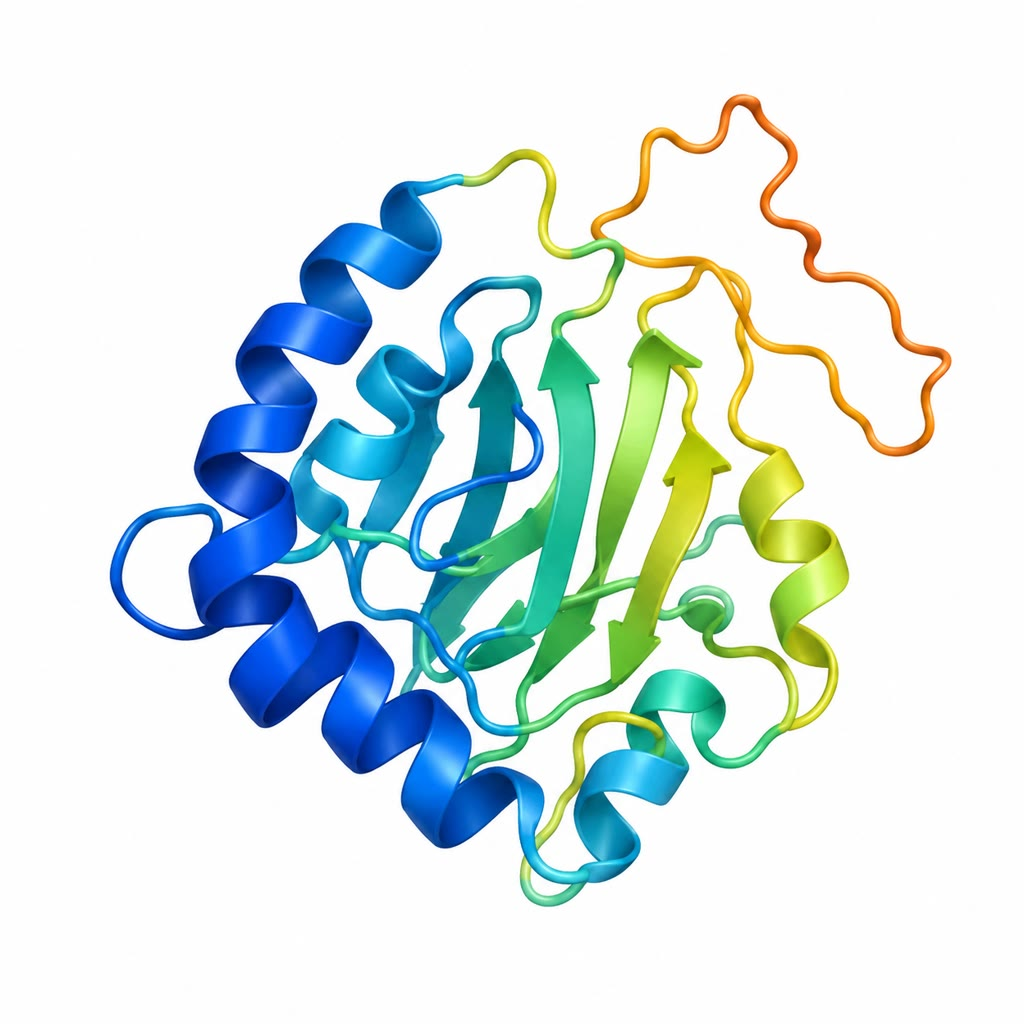
\includegraphics[width=0.36\linewidth]{images/book5/ai/b5-05-alphafold.jpg}\hspace{0.04\linewidth}
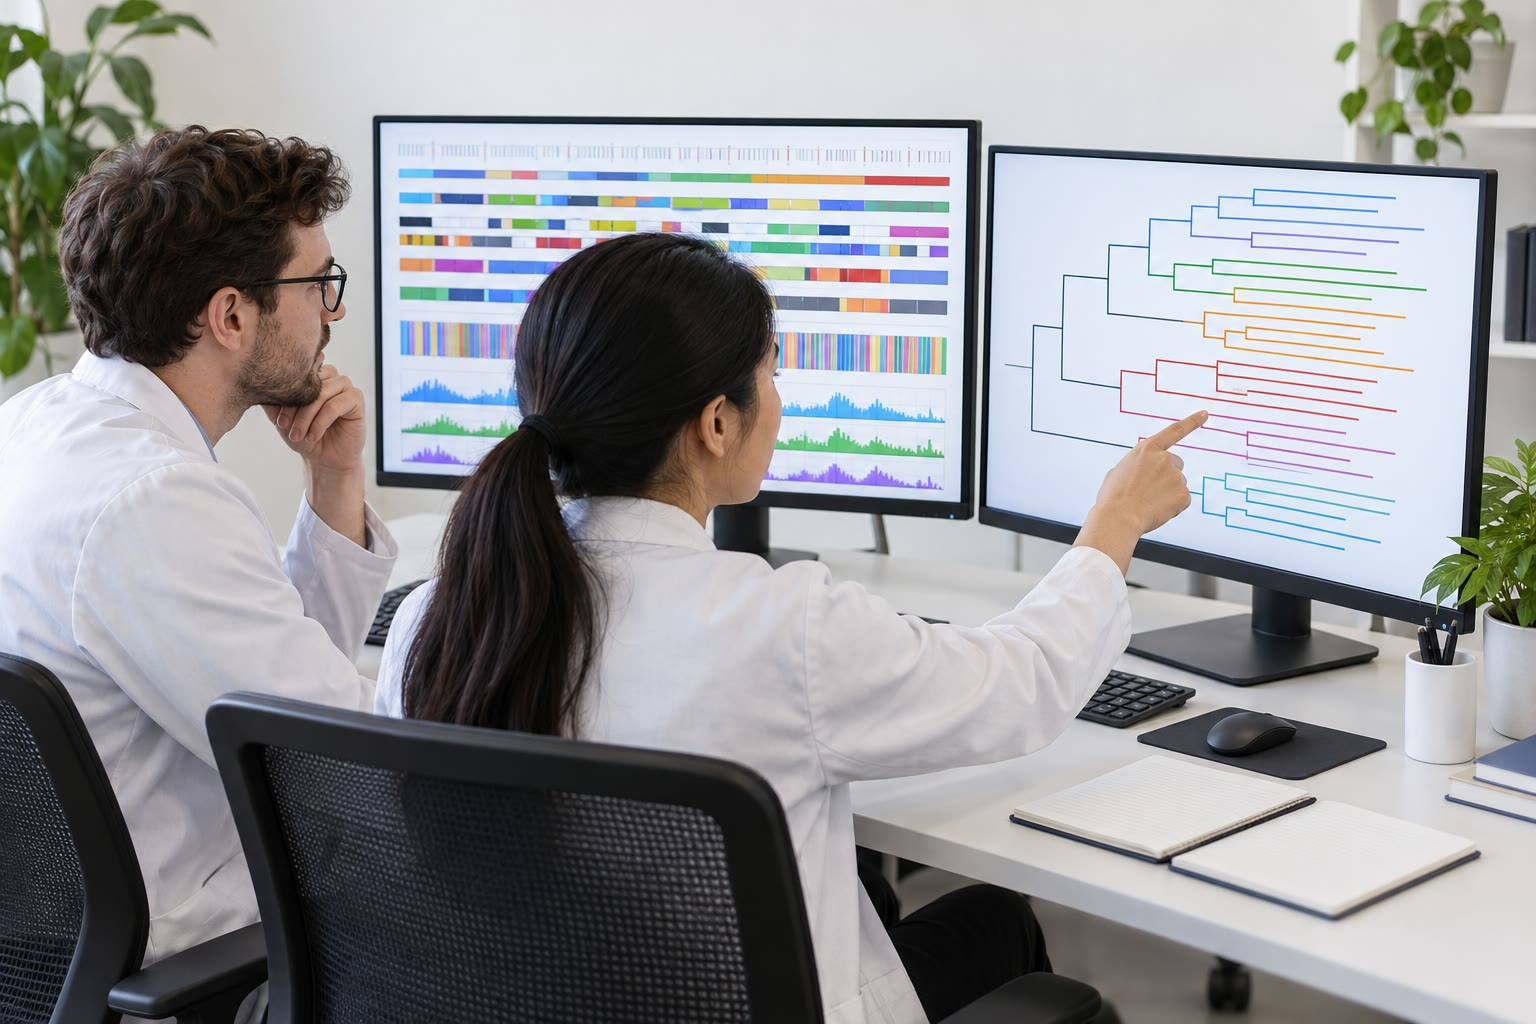
\includegraphics[width=0.54\linewidth]{images/book5/ai/b5-05-bioinformatics-lab.jpg}

{\small Links: een voorspelde eiwitstructuur, gekleurd naar het
vertrouwen van het model, van hoog (blauw) tot laag (oranje) in een
wanordelijke lus. Rechts: een bio-informaticakantoor --- genoombrowsers
en bomen op de schermen, en geen natte werkbank te bekennen.}
\end{omfigure}

\begin{remark}[De grenzen van de gevolgtrekking]\label{rem:b3:bioinformatics:limits}
De meeste functionele \omterm{def:b3:genomics:assembly}{annotaties} in de databanken zijn nooit getoetst;
zij zijn overgenomen van een homoloog, die op haar beurt door
overname was geannoteerd. Fouten planten zich voort en
vermenigvuldigen zich, en een verkeerde \omterm{def:b3:genomics:assembly}{annotatie} op een goed verbonden
eiwit kan een hele familie besmetten. De remedies zijn de bovenstaande:
onderscheid orthologie van homologie, lees de \omterm{def:b3:bioinformatics:alignment}{uitlijning}, zoek de
katalytische residuen, en onthoud dat ``hypothetisch eiwit'' een eerlijk
etiket is dat een derde van de genen in de meeste genomen nog verdient.
\end{remark}

\section{Opgaven}

\begin{exercise}[$\star$]\label{exo:b3:bioinformatics:1}
Definieer globale en \omterm{def:b3:bioinformatics:alignment}{lokale uitlijning} en geef voor elk één biologische
situatie die erom vraagt.
\end{exercise}

\begin{exercise}[$\star$]\label{exo:b3:bioinformatics:2}
Vul de tabel van Needleman--Wunsch voor AGC tegen AAC in met
overeenkomst $+1$, verschil $-1$, hiaat $-1$, en geef de optimale
\omterm{def:b3:bioinformatics:alignment}{uitlijning} en de score.
\end{exercise}

\begin{exercise}[$\star$]\label{exo:b3:bioinformatics:3}
In BLOSUM62 scoort tryptofaan--tryptofaan $+11$ en leucine--leucine
$+4$. Leg met de log-oddsformule uit waarom de identiteit van het
zeldzamere residu meer waard is.
\end{exercise}

\begin{exercise}[$\star$]\label{exo:b3:bioinformatics:4}
Wat is een E-waarde? Een zoekactie levert een treffer met $E = 3$ op.
Wat betekent dat getal, en is de treffer een homoloog?
\end{exercise}

\begin{exercise}[$\star\star$]\label{exo:b3:bioinformatics:5}
Een zoekvraag van \num{400} residuen wordt doorzocht tegen
$2\times 10^{11}$ residuen. Bereken de E-waarde van treffers met
\omterm{thm:b3:bioinformatics:evalue}{bitscores} $45$, $55$ en $65$. Welke \omterm{thm:b3:bioinformatics:evalue}{bitscore} geeft $E = 10^{-3}$? Hoe
verandert het antwoord als de zoekvraag \num{40} residuen lang is?
\end{exercise}

\begin{exercise}[$\star\star$]\label{exo:b3:bioinformatics:6}
Bereken de \omterm{def:b3:bioinformatics:motif}{informatie-inhoud} van een \omterm{def:b3:bioinformatics:motif}{motief} waarvan de vier posities
basenfrequenties (A, C, G, T) van $(1,0,0,0)$, $(0.5,0,0.5,0)$,
$(0.25,0.25,0.25,0.25)$ en $(0.7,0.1,0.1,0.1)$ hebben. Hoeveel
toevallige treffers heeft het in een genoom van \qty{4.6}{Mb}?
\end{exercise}

\begin{exercise}[$\star\star$]\label{exo:b3:bioinformatics:7}
Leg uit waarom affiene hiaatstraffen realistischer zijn dan lineaire,
en waarom zowel een zeer hoge als een zeer lage straf op het openen van
een hiaat slechte \omterm{def:b3:bioinformatics:alignment}{uitlijningen} geeft.
\end{exercise}

\begin{exercise}[$\star\star$]\label{exo:b3:bioinformatics:8}
Een BLAST-zoekactie van een menselijk eiwit tegen een vliegendatabank
geeft een beste treffer met $E = 10^{-30}$ die de residuen 50--180 van
de zoekvraag van \num{600} residuen beslaat. Is het vliegeneiwit de
\omterm{def:b3:genomics:comparative}{ortholoog} van het menselijke? Welke aanvullende toets ligt voor de
hand?
\end{exercise}

\begin{exercise}[$\star\star$]\label{exo:b3:bioinformatics:9}
Waarom sporen profielmethoden homologen op die de paarsgewijze
\omterm{def:b3:bioinformatics:alignment}{uitlijning} mist? Geef een voorbeeld van een kolompatroon dat een
\omterm{def:b3:bioinformatics:msa}{profiel} vat en één enkele sequentie niet.
\end{exercise}

\begin{exercise}[$\star\star\star$]\label{exo:b3:bioinformatics:10}
Laat zien dat onder een scoringsschema met positieve \omterm{prop:b3:bioinformatics:logodds}{verwachte score} de
\omterm{def:b3:bioinformatics:alignment}{lokale uitlijning} volgens Smith--Waterman van twee lange willekeurige
sequenties een score heeft die lineair met hun lengte groeit, en leg
uit waarom de theorie van de E-waarde daardoor faalt. Wat betekent dit
voor het uitlijnen van DNA met overeenkomst $+1$ en verschil $-1$ bij
een GC-gehalte van \qty{60}{\%}?
\end{exercise}

\begin{exercise}[$\star\star\star$]\label{exo:b3:bioinformatics:11}
De tabel van Needleman--Wunsch vergt $mn$ geheugencellen; voor twee
chromosomen van \qty{100}{Mb} is dat $10^{16}$. Beschrijf twee ideeën
waarmee genoomuitlijners dat vermijden (\omterm{def:b3:bioinformatics:blast}{seeds} en ketenen; banden), en
wat elk daarvan opgeeft.
\end{exercise}

\begin{exercise}[$\star\star\star$]\label{exo:b3:bioinformatics:12}
Een HMM voor het vinden van genen bij bacteriën heeft toestanden voor
de drie codonposities en voor niet-coderend DNA. Leg uit hoe het model
coderende van niet-coderende sequentie kan onderscheiden zonder enige
informatie over stopcodons (denk aan het codongebruik), en waarom
dezelfde aanpak in een menselijk genoom veel moeilijker is.
\end{exercise}

\section{Vraagstuk: een sequentie uit de diepzee}

\begin{problem}[{Weekendvraagstuk --- een onbekend eiwit met de hand
uitgelijnd, tegen de databanken doorzocht met berekening van zijn
significantie, zijn regulerende motief in bits gewogen, en zijn gen
getoetst aan de statistiek van toevallige open leesramen, met als
besluit de E-waarde van de beste treffer, het aantal bits dat een
plaats nodig heeft en de lengte die een leesraam moet hebben om
geloofd te worden}]
\label{pb:b3:bioinformatics:1}
Gegevens: een eiwit van \num{300} residuen uit een diepzeeworm.
Eiwitdatabank: $1.2\times 10^{11}$ residuen. Genoom van de worm:
\qty{1.6}{Gb}, \qty{38}{\%} GC. Scoring voor \omterm{def:b3:bioinformatics:alignment}{uitlijningen} met de hand:
overeenkomst $+1$, verschil $-1$, hiaat $-1$. \omterm{thm:b3:bioinformatics:evalue}{Bitscore} van de beste
BLAST-treffer: $92$; van de tiende treffer: $38$.

\medskip
\noindent\textbf{Deel I --- Met de hand.}
\begin{enumerate}
  \item Lijn de peptiden KQT en KAQT uit met de recursie van
        Needleman--Wunsch: schrijf de tabel op en geef de optimale
        \omterm{def:b3:bioinformatics:alignment}{uitlijning} en de score.
  \item Doe hetzelfde met Smith--Waterman (lokaal) voor GATCAT tegen
        ACAT: zoek de beste \omterm{def:b3:bioinformatics:alignment}{lokale uitlijning} en haar score.
  \item Hoeveel celbewerkingen kost een \omterm{def:b3:bioinformatics:alignment}{globale uitlijning} van het
        eiwit van \num{300} residuen tegen een eiwit van \num{450}
        residuen? En tegen de hele databank?
  \item Als een computer $10^{9}$ bewerkingen per seconde uitvoert, hoe
        lang duurt de volledige databankuitlijning van vraag 3 dan?
        Waarom wordt in plaats daarvan \omterm{def:b3:bioinformatics:blast}{BLAST} gebruikt?
  \item Een identiteitsscore in BLOSUM62 is $+4$ voor alanine ($p_{A} =
        0.074$) en $+11$ voor tryptofaan ($p_{W} = 0.013$). Bereken met
        $\lambda = 0.347$ (eenheden van een halve bit) de
        doelfrequenties $q_{AA}$ en $q_{WW}$, en de verhouding
        $q/p^{2}$ voor elk. Geef de betekenis.
  \item Twee eiwitten delen \qty{24}{\%} identiteit over $250$ residuen.
        Zeg waarom identiteit alleen hier de homologie niet kan
        beslechten en wat dat wel zou doen.
\end{enumerate}

\medskip
\noindent\textbf{Deel II --- De zoekactie.}
\begin{enumerate}[resume]
  \item Bereken $mn$ voor de zoekvraag tegen de databank, en
        $\log_{2}(mn)$.
  \item Bereken de E-waarde van de beste treffer ($S' = 92$) en van de
        tiende treffer ($S' = 38$).
  \item Welke \omterm{thm:b3:bioinformatics:evalue}{bitscore} komt bij deze zoekactie overeen met
        $E = 10^{-3}$? En met $E = 1$?
  \item Dezelfde beste treffer wordt gevonden wanneer de databank tot
        $1.2\times 10^{12}$ residuen is gegroeid. Wat is haar E-waarde?
  \item De tiende treffer lijnt de residuen 200--260 van de zoekvraag
        uit met \qty{40}{\%} identiteit over $60$ residuen. Zeg met de
        E-waarde of dit bewijs van homologie is, en wat een
        profielzoekactie zou kunnen toevoegen.
  \item De beste treffer is een menselijk kinase, uitgelijnd over de
        residuen 10--290. Zijn beste treffer in het eiwitbestand van de
        worm is de zoekvraag. Wat stelt deze wederzijdse toets vast, en
        wat niet?
\end{enumerate}

\medskip
\noindent\textbf{Deel III --- Een \omterm{def:b3:bioinformatics:motif}{motief}.}
\begin{enumerate}[resume]
  \item Stroomopwaarts van het gen ligt een kandidaat-bindingsplaats
        voor een transcriptiefactor van acht posities met
        \omterm{def:b3:bioinformatics:motif}{informatie-inhouden} $2, 2, 1.6, 2, 0.8, 1.2, 0.4, 0.3$ bits.
        Wat is $R$ in totaal?
  \item Hoeveel toevallige treffers heeft het \omterm{def:b3:bioinformatics:motif}{motief} in het genoom van
        \qty{1.6}{Gb} (beide strengen, $3.2\times 10^{9}$ posities)?
  \item De factor reguleert ongeveer $200$ genen. Hoeveel bits zou een
        \omterm{def:b3:bioinformatics:motif}{motief} nodig hebben om in dit genoom $200$ plaatsen alleen aan
        te wijzen?
  \item Hoeveel van het tekort zou een tweede, aangrenzend \omterm{def:b3:bioinformatics:motif}{motief} van
        $8$ bits kunnen leveren, als de twee binnen een vaste
        tussenafstand samen moeten voorkomen?
  \item Een positie met frequenties $(0.5, 0.5, 0, 0)$ voor (A, C, G,
        T): bereken haar entropie en haar \omterm{def:b3:bioinformatics:motif}{informatie-inhoud}.
  \item Leg met het informatieargument uit waarom bacteriële
        transcriptiefactoren doorgaans langere en beter geconserveerde
        plaatsen hebben dan eukaryote.
\end{enumerate}

\medskip
\noindent\textbf{Deel IV --- Het gen zelf.}
\begin{enumerate}[resume]
  \item Wat is in willekeurig DNA met gelijke basensamenstelling de
        kans dat een codon een stopcodon is? Wat is het verwachte
        aantal codons voordat er een stopcodon verschijnt (een
        geometrische verdeling)?
  \item Het genoom van de worm is voor \qty{38}{\%} GC. Herbereken met
        de werkelijke basenfrequenties de kans dat een willekeurig
        codon een stopcodon is (TAA, TAG, TGA), en de verwachte lengte
        van het leesraam. Welke kant op duwt een laag GC-gehalte het
        vinden van genen?
  \item Wat is de kans dat een willekeurig open leesraam minstens $100$
        codons lang is? En minstens $300$?
  \item In het genoom van \qty{1.6}{Gb} geven zes leesramen op twee
        strengen ongeveer $3.2\times 10^{9}$ codonbeginpunten. Hoeveel
        willekeurige open leesramen van minstens $100$ codons zijn te
        verwachten? En van minstens $300$?
  \item Leg uit waarom ``open leesraam langer dan $100$ codons'' bij een
        bacterie een bruikbare genzoeker is en in dit genoom niet, en
        wat een eukaryote genzoeker in plaats daarvan gebruikt.
  \item Het gen van de worm heeft zes exons van gemiddeld \qty{150}{bp}.
        Leg uit hoe \omterm{def:b3:genomics:ngs}{reads} uit RNA-sequencing de exonstructuur
        vaststellen die de genoomsequentie alleen onduidelijk laat.
  \item Vat samen: de E-waarde van de beste treffer (vraag~8), het
        aantal bits dat nodig is om $200$ plaatsen aan te wijzen
        (vraag~15), en het verwachte aantal willekeurige leesramen van
        $300$ codons in het genoom (vraag~22).
\end{enumerate}
\end{problem}
